\newpage
\hypertarget{treeToModel tex}{}
\subsection{The textual transformation rules}
\texHeader

Please note that we have assumed a basic understanding of TGGs, specifically those about constructing each scope in a rule, and how to use Eclipse efficiently
with eMoflon's auto-completion feature. If you find this section challenging, we recommend first working through Part IV to cover TGG fundamentals.

\begin{itemize}

\subsubsection{FolderToLibraryRule} % ---------------------------------

\item[$\blacktriangleright$] Return and expand the \texttt{DictionaryCodeAdapter} TGG package and right-click on the \texttt{Rules} folder. Create your first
rule by navigating to ``New/TGG Rule," naming it \texttt{Folder\-To\-Lib\-rary\-Rule}.

\item[$\blacktriangleright$] All this rule needs to do is create a \texttt{Folder} (i.e., ``myLibrary'') together with its equivalent \texttt{Library}, and
establish a correspondence link between them. Edit your rule until it resembles Fig.~\ref{eclipse:FolderToLibraryRule}.

\vspace{0.5cm}

\begin{figure}[htbp]
\begin{center}
  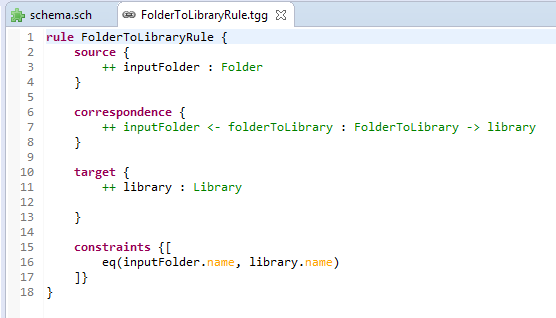
\includegraphics[width=\textwidth]{eclipse_FolderToLibraryRule}
  \caption{The TGG transformation begins with this rule.}
  \label{eclipse:FolderToLibraryRule}
\end{center}
\end{figure}

\vspace{-0.5cm}

\subsubsection{ForAllShelfRule} % ---------------------------------

\item[$\blacktriangleright$] Let's use some elements from the previous rule to help us define how to handle creating shelves for our library. Copy and paste the
required context elements from \texttt{FolderToLibraryRule} in a new \texttt{ForAllShelfRule}, adding a new \texttt{shelfFolder} and \texttt{shelf} as depicted
in Fig.~\ref{eclipse:ForAllShelvesRule}.

\vspace{0.5cm}

\begin{figure}[htbp]
\begin{center}
  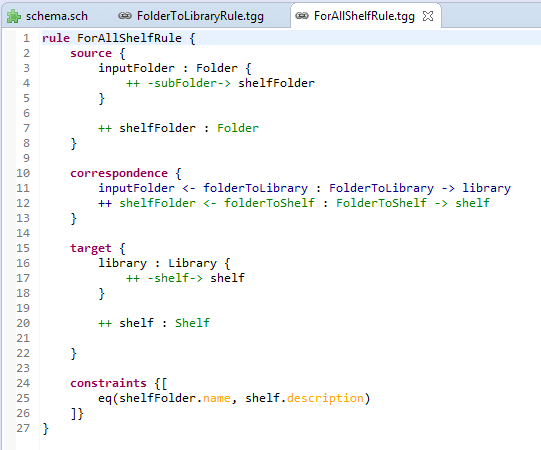
\includegraphics[width=0.9\textwidth]{eclipse_ForAllShelfRule}
  \caption{\texttt{ForAllShelfRule}}
  \label{eclipse:ForAllShelvesRule}
\end{center}
\end{figure}

\item[$\blacktriangleright$] Add the new correspondence type to your \texttt{schema} (Fig.~\ref{eclipse:updatedSchema}).

\vspace{0.5cm}

\begin{figure}[h!]
\begin{center}
  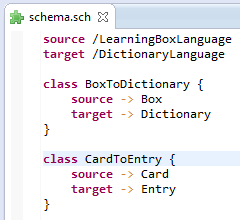
\includegraphics[width=0.7\textwidth]{eclipse_updatedSchema}
  \caption{Updated TGG \texttt{schema}}
  \label{eclipse:updatedSchema}
\end{center}
\end{figure}

\newpage

Now that we can assume the primary library and shelf containers exist, we can handle the dictionary \texttt{File} elements. We know from our generated
tree model that a dictionary will always have a title node, but we're unsure if an author will be included, and there's no way to know how many entries are
involved. Therefore, we should create at least three different rules to handle this stage of the transformation. 

\subsubsection{NodeToDictionaryRule} % ---------------------------------

\item[$\blacktriangleright$] Create a rule name \texttt{NodeToDictionaryRule} as indicated in Fig.~\ref{eclipse:NodeToDictionaryRule}.

\vspace{0.5cm}

\begin{figure}[htbp]
\begin{center}
  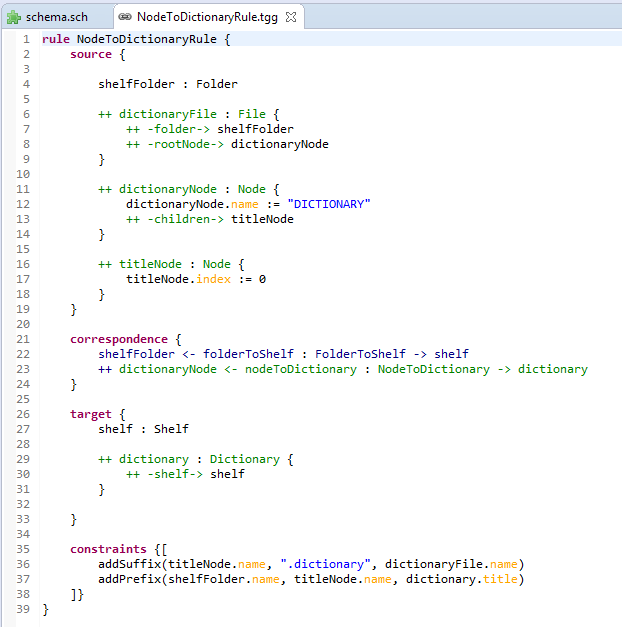
\includegraphics[width=\textwidth]{eclipse_NodeToDictionaryRule}
  \caption{\texttt{NodeToDictionaryRule} handling only \texttt{titleNode}s}
  \label{eclipse:NodeToDictionaryRule}
\end{center}
\end{figure}

\newpage

\item[$\blacktriangleright$] As you can see, this rule demands that a \texttt{shelfFolder} and \texttt{shelf} already exist before executing, implying that this
rule can only be called after executing \texttt{ForAllShelfRule}. An attribute constraint is used with \texttt{titleNode} to ensure that the correct child
\texttt{Node} is matched from \texttt{dictionaryNode}, and not accidentally to an author or entry node, which will have different indices.

\item[$\blacktriangleright$] This rule also imposes two constraints for attribute manipulation. We need to add the name of the shelf as a prefix to the title
node's name to get the dictionary's title (i.e., ``english'' + ``numbers1-10''). Similarly, the second constraint appends \texttt{.dictionary} to
\texttt{titleNode.name} to get the file name of the dictionary.

\subsubsection{ForAllEntryRule} % ---------------------------------

\item[$\blacktriangleright$] Let's handle \texttt{Entry} elements next. Create \texttt{ForAllEntryRule} so that it closely resembles
Fig.~\ref{eclipse:ForAllEntryRule}.

\vspace{0.5cm}

You can see that this rule has three attribute constraints, one of which we haven't encountered before. The first two \texttt{eq} constraints guarantee that
an \texttt{entryNode}'s content and index values remain consistent with its equivalent \texttt{entry} in a \texttt{dictionary}. The final constraint is to
ensure that any new \texttt{entryNode}s created in the backward transformation have index values set to 2. 

\vspace{0.5cm}

Without this final constraint, all new \texttt{entryNodes} would have a default 0 index value, and
could be mistaken as \texttt{titleNodes} as described in the previous \texttt{NodeToDictionaryRule}, causing the entire transformation to fail.

\newpage

\begin{figure}[htbp]
\begin{center}
  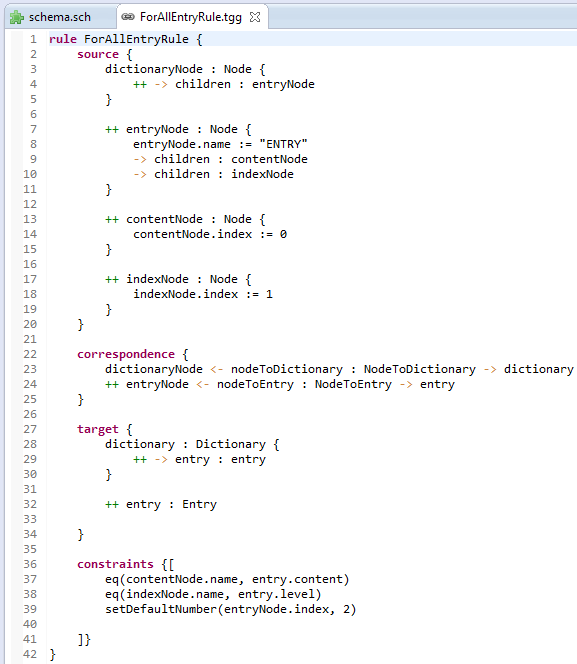
\includegraphics[width=\textwidth]{eclipse_ForAllEntryRule}
  \caption{\texttt{ForAllEntryRule}}
  \label{eclipse:ForAllEntryRule}
\end{center}
\end{figure}

\vspace{0.5cm}

The last thing we need to specify is how to handle \texttt{author}s. Transforming an \texttt{authorNode} to an \texttt{author} isn't as simple as
an \texttt{entryNode}, where you create an \texttt{entry} every time. Instead, we have to account for the possibility of a single author
for multiple dictionaries in a \texttt{Library}. While some users may not care about having redundant information, why not also provide a rule for users
who want to enforce unique authors in a \texttt{Library}?

\subsubsection{NewAuthorRule} % ---------------------------------

\item[$\blacktriangleright$] Create \texttt{NewAuthorRule}, and complete it as depicted in Fig.~\ref{eclipse:ForAllNewAuthorRule}. This is a one-to-one
correspondence rule, where every \texttt{authorNode} creates a new \texttt{author}. If this rule is used in a transformation, one might end up with
multiple authors with the same email address.

\vspace{0.5cm}

\begin{figure}[htbp]
\begin{center}
  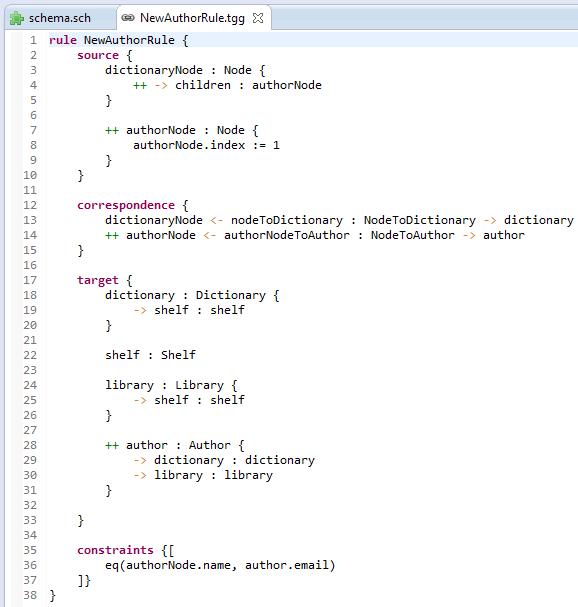
\includegraphics[width=\textwidth]{eclipse_NewAuthorRule}
  \caption{Creating new authors in \texttt{NewAuthorRule}}
  \label{eclipse:ForAllNewAuthorRule}
\end{center}
\end{figure}

\newpage

\subsubsection{ExistingAuthorRule} % ---------------------------------

\item[$\blacktriangleright$] Similarly, create \texttt{ExistingAuthorRule} as specified in Fig.~\ref{eclipse:ForExistingAuthorRule}. You should be able to
copy and paste the majority of the previous rule. In fact, the only thing you need to change are two small characters in front of \texttt{author} and its
\texttt{dictionary} reference, forcing the rule to find an existing \texttt{author}, if possible.

\vspace{0.5cm}

\begin{figure}[htbp]
\begin{center}
  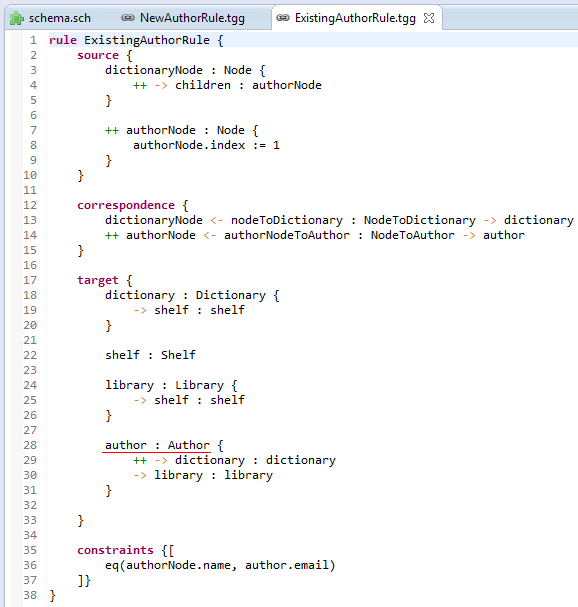
\includegraphics[width=\textwidth]{eclipse_ExistingAuthorRule}
  \caption{Checking for existing authors in \texttt{ExistingAuthorRule}}
  \label{eclipse:ForExistingAuthorRule}
\end{center}
\end{figure}

\newpage

\item[$\blacktriangleright$] Great work! You have now specified five different rules to handle a bidirectional text-to-model transformation! For confirmation,
your final schema and package explorer should now resemble Fig.~\ref{eclipse:schemaFinal}.

\vspace{0.5cm}

\begin{figure}[htbp]
\begin{center}
  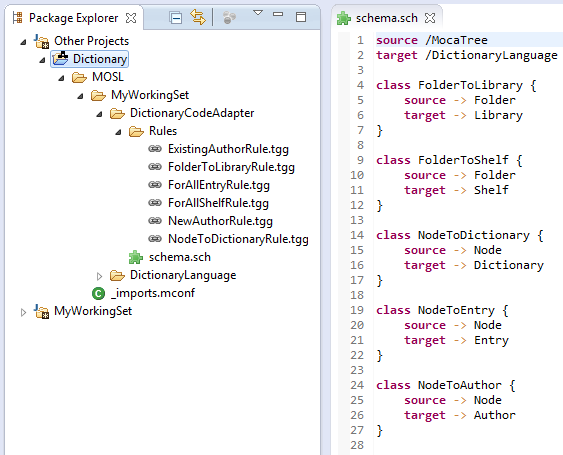
\includegraphics[width=\textwidth]{eclipse_finalSchema}
  \caption{Your final \texttt{rules} project structure and \texttt{schema}}
  \label{eclipse:schemaFinal}
\end{center}
\end{figure}

\vspace{0.5cm}

\item[$\blacktriangleright$] Given that everything has been done correctly, and MOSL hasn't reported any errors, build your TGG transformation. If problems
arise, be sure to double-check your files for spelling or other mistakes.

\end{itemize}
